\chapter{Machine Learining}
\label{ch:MachineLearning}

Before diving into the description of the unsupervised algorithms used for the development of this thesis work presented in \autoref{ch:Unsupervised}, this chapter aims to be an introduction of \emph{Machine Learning} (\gls{ml}) in general.

An early but useful definition of Machine Learning was given by Arthur Samuel in 1959: \quoted{\emph{Machine learning is the field of study that gives computers the ability to learn without being explicitly programmed.}} A more recent definition is the following, from Tom Mitchell: \quoted{\emph{A computer program is said to learn from experience E with respect to some task T and some performance measure P, if its performance on T, as measured by P, improves with experience E.}} \citepage{hands-on-geron2022}{4}

So, in general, the ingredients of \gls{ml} are:
\begin{itemize}
    \item some data linked to some task
    \item a task to be performed
    \item an algorithm that learns how to perform the task on specific data
\end{itemize}

The data are usually preprocessed before giving them to the algorithm. The processed data are called \emph{features}. This is a generic term that refers to the information content of the data.
For example, if the data are recordings of temperatures over time, the features could be the mean, the standard deviation, the minimum, and the maximum of the temperature or, in some cases if the algorithm is able to learn directly from them, the raw data themself.

The tasks can be divided into main categories:
\begin{itemize}
    \item regression: the algorithm is trained to measure the relation between the value of output variables and corresponding values of other input variables;
    \item classification: the algorithm is trained to assign a label to a new instance, based on the training dataset of labeled instances;
    \item clustering: the algorithm is trained to group similar instances into clusters.
    \item anomaly detection: the algorithm is trained to identify instances that are different from known previous instances.
\end{itemize}

\section{Regression}
\label{sec:Regression}


\subsection{Least Squares}
\label{subsec:LS}

Lets consider a set of $m$ observations of a variable $y \in \mathbb{R}^{n_y}$ (output features) that depends on a variable $x \in \mathbb{R}^{n_x}$ (input features) and a set of $n_f \cdot n_y$ parameters $\theta \in \mathbb{R}^{n_f \times n_y}$.

Suppose to know that the output features are linked to the input features with $n_f$ functions linear in the parameters $\theta$, so that:
\begin{multline*}
    \begin{bmatrix}
        y_1 & y_2 & \dots & y_{n_y} 
    \end{bmatrix}
    =\\
        \begin{bmatrix}
            f_1(x_1, \dots, x_{n_x}) & f_2(x_1, \dots, x_{n_x}) & \dots & f_{n_f}(x_1, \dots, x_{n_x}) \\
        \end{bmatrix}
        \cdot
        \begin{bmatrix}
            \theta_{1,1}  & \dots & \theta_{1,n_y} \\
            \theta_{2,1}  & \dots & \theta_{2,n_y} \\
            \vdots & \ddots & \vdots \\
            \theta_{n_f,1}  & \dots & \theta_{n_f,n_y} \\
        \end{bmatrix}
\end{multline*}

Where all the $f_i$ are any known functions, $y_i$ and $x_i$ are known data and $\theta_{i,j}$ are the parameters to be found.

Considering the $m$ observations, the previous equation can be extended as:

\begin{multline*}
    \begin{bmatrix}
        y_{1,1} & y_{1,2} & \dots & y_{1,n_y} \\
        y_{2,1} & y_{2,2} & \dots & y_{2,n_y} \\
        \vdots & \ddots & \vdots \\
        y_{m,1} & y_{m,2} & \dots & y_{m,n_y} \\
    \end{bmatrix}
    =\\
        \begin{bmatrix}
            f_1(x_{1,1}, \dots, x_{1,n_x}) & \dots & f_{n_f}(x_{1,1}, \dots, x_{1,n_x}) \\
            f_1(x_{2,1}, \dots, x_{2,n_x}) & \dots & f_{n_f}(x_{2,1}, \dots, x_{2,n_x}) \\
            \vdots  & \ddots & \vdots \\
            f_1(x_{m,1}, \dots, x_{m,n_x}) & \dots & f_{n_f}(x_{m,1}, \dots, x_{m,n_x}) \\
        \end{bmatrix}
        \cdot
        \begin{bmatrix}
            \theta_{1,1}  & \dots & \theta_{1,n_y} \\
            \theta_{2,1}  & \dots & \theta_{2,n_y} \\
            \vdots & \ddots & \vdots \\
            \theta_{n_f,1}  & \dots & \theta_{n_f,n_y} \\
        \end{bmatrix}
\end{multline*}


Rewriting the previous equation in a more compact form:

\begin{equation}
    \begin{bmatrix}
        \vect{y}_1 \\
        \vect{y}_2 \\
        \vdots \\
        \vect{y}_m \\
    \end{bmatrix}
    =
    \begin{bmatrix}
        f_1(\vect{x}_1) & f_2(\vect{x}_1) & \dots & f_{n_f}(\vect{x}_1) \\
        f_1(\vect{x}_2) & f_2(\vect{x}_2) & \dots & f_{n_f}(\vect{x}_2) \\
        \vdots & \ddots & \vdots \\
        f_1(\vect{x}_m) & f_2(\vect{x}_m) & \dots & f_{n_f}(\vect{x}_m) \\
    \end{bmatrix}
    \cdot
    \begin{bmatrix}
        \theta_{1,1}  & \dots & \theta_{1,n_y} \\
        \theta_{2,1}  & \dots & \theta_{2,n_y} \\
        \vdots & \ddots & \vdots \\
        \theta_{n_f,1}  & \dots & \theta_{n_f,n_y} \\
    \end{bmatrix}
\end{equation}

That, in the most compact form, becomes:

\begin{equation}
    \vect{Y} = \vect{\Phi}(\vect{X}) \cdot \vect{\Theta}
\end{equation}

In close form, there is a solution $\vect{\Theta_{LS}}$, for estimating the parameters that minimize the error between the estimated output $\vect{Y_{LS}} = \vect{\Phi(\vect{X})}\vect{\Theta_{LS}}$ and the real output $\vect{Y_{}}$, that is known. Let's see, in an intuitive way:
\begin{eqnarray}
    \vect{Y} &=& \vect{\Phi}(\vect{X}) \cdot \vect{\Theta_{LS}} \\
    \vect{\Phi}(\vect{X})^T\vect{Y} &=& \underbrace{\vect{\Phi}(\vect{X})^T\vect{\Phi}(\vect{X})}_{\text{square}}\cdot \vect{\Theta_{LS}}\\
    (\vect{\Phi}(\vect{X})^T\vect{\Phi}(\vect{X}))^{-1}\vect{\Phi}(\vect{X})^T\vect{Y} &=& \vect{\Theta_{LS}}\\
    \text{pinv}(\vect{\Phi}(\vect{X}))\vect{Y} &=& \vect{\Theta_{LS}} \label{eq:LS}
\end{eqnarray}

In fact, it is known that $\vect{\Theta_{LS}} = \text{pinv}(\vect{\Phi}(\vect{X}))\vect{Y}$ is the solution of the following minimization problem:

\begin{equation}
    \vect{\Theta_{LS}} = \argmin{\vect{\Theta} \in \mathbb{R}^{n_f \times n_y}}{\norm{\vect{Y}-\vect{\Phi}(\vect{X})\vect{\Theta}}_2^2}
\end{equation}

That is why this method is called \emph{Least Squares} (\gls{ls}). It is proven that if the data $\vect{Y}$ affected my white noise, and the data $\vect{X}$ are known precisely, the solution converges to the real parameters $\vect{\Theta}_{\text{true}}$ when the number of observations $m$ goes to infinity.
\begin{equation}
    \lim_{m \to \infty} \vect{\Theta_{LS}} = \vect{\Theta}_{\text{true}}
\end{equation}

Is this considered machine learning? Yes, even being just a simple implementation of linear algebra, once programmed in a computer, it qualifies as the (simplest) machine learning algorithm because fitting new data does not require any human intervention. Let's see an example. Suppose to have 400 data points, shown in \autoref{fig:LinearRegressiondData}, of the variable $x$, $y_1$ and $y_2$ sampled with noise, that we call Fature 1, Feature 2 and Feature 3, respectively. Suppose that it is known that the output features are linked to the input feature with a linear combination of the functions $e^x$, $x^3$, $\cos(x)$, $\sin(x)$ and $\cos^3(x)$, but the parameters $\theta$ are unknown:

\begin{eqnarray}
    y_1 &=& \theta_{1,1} e^x + \theta_{2,1} x^3 + \theta_{3,1} \cos(x) + \theta_{4,1} \sin(x) + \theta_{5,1} \cos^3(x) \\
    y_2 &=& \theta_{1,2} e^x + \theta_{2,2} x^3 + \theta_{3,2} \cos(x) + \theta_{4,2} \sin(x) + \theta_{5,2} \cos^3(x)
\end{eqnarray}

\begin{figure}
    \centering
    \begin{subfigure}{0.49\textwidth}  % <----
        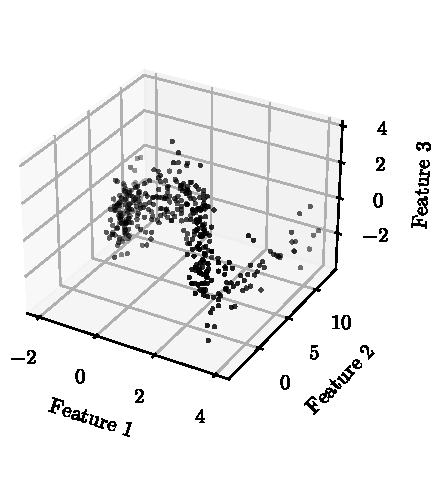
\includegraphics[width=\textwidth]{images/MachineLearning/LinearRegressiondData.pdf}
        \caption{400 data points}
        \label{fig:LinearRegressiondData}
    \end{subfigure}
    \begin{subfigure}{0.49\textwidth}  % <----
        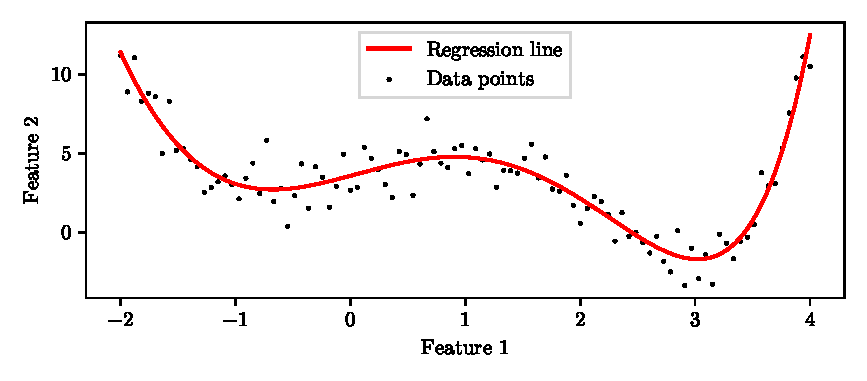
\includegraphics[width=\textwidth]{images/MachineLearning/LinearRegression.pdf}
        \caption{data points and the fitted curve}
        \label{fig:LinearRegression}
    \end{subfigure}
    \caption{Least square regression example}
\end{figure}

rearranging in matrix form: 
\begin{equation}
    \underbrace{\begin{bmatrix}
        y_{1,1} & y_{1,2} \\
        y_{2,1} & y_{2,2} \\
        \vdots & \vdots \\
        y_{m,1} & y_{m,2} \\
    \end{bmatrix}}_{\vect{Y}}
    =
    \underbrace{\begin{bmatrix}
        e^{x_1} & x_1^3 & \cos(x_1) & \sin(x_1) & \cos^3(x_1) \\
        e^{x_2} & x_2^3 & \cos(x_2) & \sin(x_2) & \cos^3(x_2) \\
        \vdots & \vdots & \vdots & \vdots & \vdots \\
        e^{x_m} & x_m^3 & \cos(x_m) & \sin(x_m) & \cos^3(x_m) \\
    \end{bmatrix}}_{\vect{\Phi}(\vect{X})}
    \cdot
    \underbrace{\begin{bmatrix}
        \theta_{1,1}  & \theta_{1,2} \\
        \theta_{2,1}  & \theta_{2,2} \\
        \theta_{3,1}  & \theta_{3,2} \\
        \theta_{4,1}  & \theta_{4,2} \\
        \theta_{5,1}  & \theta_{5,2} \\
    \end{bmatrix}}_{\vect{\Theta}}
\end{equation}

applying the \gls{ls} solution from \autoref{eq:LS}, we obtain:
\begin{equation*}
    \vect{\Theta_{LS}} = \text{pinv}(\vect{\Phi}(\vect{X}))\vect{Y} = 
    \begin{bmatrix}
        +1.997 & -0.004 \\
        -1.498 & +0.003 \\
        +1.332 & -0.018 \\
        -0.005 &  +0.999 \\
        -0.032 & +1.035 
    \end{bmatrix}
\end{equation*}

that is quite close to the real parameters used to generate the data:
\begin{equation*}
    \vect{\Theta}_{\text{true}} = 
    \begin{bmatrix}
        +2.0 & +0 \\
        -1.5 & +0 \\
        +1.3 & +0 \\
        +0.0 & +1 \\
        +0.0 & +1 
    \end{bmatrix}
\end{equation*}

Using the estimated parameters, it is possible to estimate the output features for new input features, the regression line is shown in \autoref{fig:LinearRegression}.

\subsubsection{Applicability}
This is an elegant closed-form solution for a regression problem, however, it has some limitations:
\begin{itemize}
    \item if the noise is not white, or it is present also in the input features, the solution is not guaranteed to converge to the real parameters;
    \item if there are nonlinearities in the parameters (for example $\sin(\theta_{1,1}x)$), the solution is not applicable;
\end{itemize}

\subsection{Gradient Descent \gls{gd}}
To overcome these limitations, another way to estimate the parameters is to use an iterative algorithm that minimizes a cost function over the parameters space. The iterations aim to update the parameters in the direction of the steepest descent of the cost function. This can be done even with nonlinearities in the data, and even if the noise is not white, but has the drawback of the risk of getting stuck in a local minimum of the cost function, starting from a random initialization.
Another limitation is the fact that a learning rate $\eta$ has to be defined, that is a parameter that defines how much the parameters are updated at each iteration. If the learning rate is too small, the algorithm will take a lot of time to converge, if it is too large, the algorithm may overshoot the minimum and avoid convergence.

In the previous closed form solution (\autoref{subsec:LS}), the hypotesis function was linear in the parameters $\vect{Y} = \vect{\Phi}(\vect{X})\cdot\vect{\Theta}$, so we can call this prediction $\vect{\hat{y}} = \vect{h}_{\vect{\Theta}}(\vect{x})$.

The cost function to be minimized is usually defined as the mean squared error between the prediction and the real data:
\begin{equation}
    \text{MSE}(\vect{X}, h_{\vect{\Theta}}) = \frac{1}{m}\sum_{i=1}^{m}(\vect{\hat{y}}_i - \vect{y}_i)^2
\end{equation}


The gradient of the cost function, used by all gradient descent algorithms, is defined as:

\begin{equation}
\nabla_{\vect{\Theta}} \text{MSE}(\vect{X}, h_{\vect{\Theta}}) = 
\begin{bmatrix}
    \frac{\partial}{\partial \theta_1} \text{MSE}(\vect{X}, h_{\vect{\Theta}}) \\
    \frac{\partial}{\partial \theta_2} \text{MSE}(\vect{X}, h_{\vect{\Theta}}) \\
    \vdots \\
    \frac{\partial}{\partial \theta_{n_f\times n_y}} \text{MSE}(\vect{X}, h_{\vect{\Theta}}) \\
\end{bmatrix}
\end{equation}

The algorithm then updates the parameters at each iteration as:
\begin{equation}
    \vect{\Theta}^{(i+1)} = \vect{\Theta}^{(i)} - \eta \nabla_{\vect{\Theta}} \text{MSE}(\vect{X}, h_{\vect{\Theta}})
\end{equation}


\subsection{Sthocastic Gradient Descent}
\label{subsec:SGD}
The \emph{Stochastic Gradient Descent} (\gls{gd}) is a variant of the \gls{gd} algorithm that computes the gradient only on one instance at each iteration, instead of on the whole dataset. This makes the algorithm much faster, but the cost function will be much more noisy, and theta will not reach a steady value but instead will oscillate around the minimum. This has the advantage of being more robust to local minimum entrapment, but the disadvantage of never reaching the minimum. To overcome this, the learning rate $\eta$ can be reduced at each iteration, but this will slow down the convergence.

\begin{figure}
    \centering
    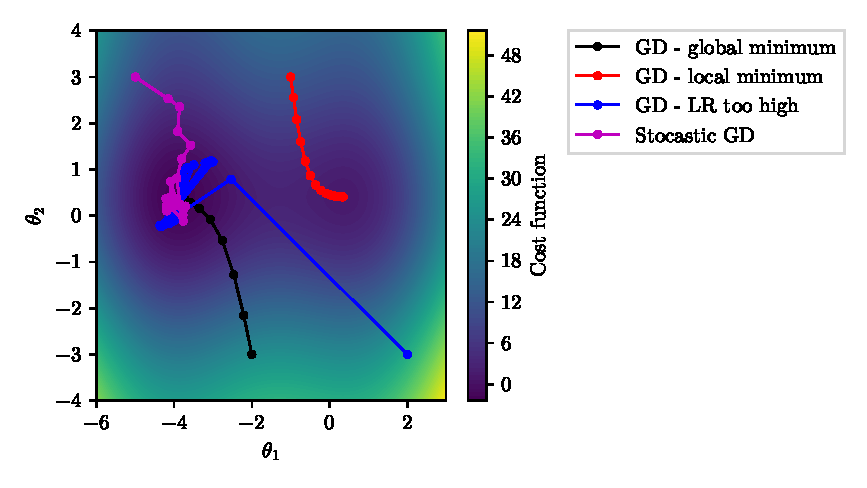
\includegraphics[width=\textwidth]{images/MachineLearning/GradientDescent.pdf}
    \caption{Gradient Descent comparison}
    \label{fig:SGD}
\end{figure}

In the \autoref{fig:SGD} it is visualized graphically what has been said about Gradient Descent.

\subsection{Avoid overfitting}
\label{subsec:overfitting}
The \gls{gd} algorithm is very powerful, but it can overfit the data. To avoid that, the problem of when to stop the iterations has to be addressed. A common way to do that is to split the dataset into a training set and a validation set. The training set is used to train the algorithm, and the validation set is used to evaluate the performance of the algorithm on new data. The training is stopped when the performance on the validation set starts to degrade, even if the performance on the training set is still improving. This is called \emph{early stopping}. In the \autoref{fig:overfitting} it is shown an example of early stopping using as metric the \emph{Root Mean Square Error} (RMSE), that is just the square root of MSE, on the validation set.

\begin{figure}
    \centering
    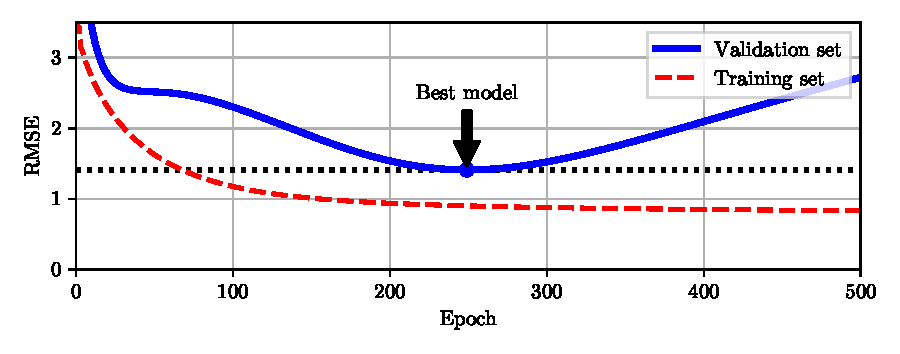
\includegraphics[width=\textwidth]{images/MachineLearning/EarlyStopping.pdf}
    \caption{Overfitting example \citepage{hands-on-geron2022}{162}}
    \label{fig:overfitting}
\end{figure}

\section{Classification}
\label{sec:Classification}
Another common task in \gls{ml} is classification. In this case, the algorithm is trained to assign a label to a new instance, based on the training dataset of labeled instances. Naively, it aims to define a set of rules that divide the space of the input features in regions, each one associated with a label. The two main approaches are \emph{hard} and \emph{soft} classification. In the former, the algorithm is trained to assign a single label to each instance, while in the latter, the algorithm is trained to output a probability for each label, and the label with the highest probability is assigned to the instance.

Classification is a \emph{supervised} learning task because the training dataset is labeled. The labels can be provided by a human or can be generated by another algorithm. Some classification algorithms are available also in the unsupervised version, where the labels are not provided, and the task is usually novelty detection.

\subsection{Support Vector Machines \gls{svm}}
\label{subsec:svm}
Support Vector Machines are simple but powerful classification algorithms that can be used both for hard and soft classification, with medium size datasets. They are based on the idea of finding the hyperplane that best divides the space of the input features into two regions, each one associated with a label.

The main drawback is that, natively, they can only be used for binary classification (two classes), but there are some extensions that allow to use of them for multiclass classification. Furthermore, as will be explained in \autoref{sec:OneClassSupportVectorMachine}, they can be used also for novelty detection (one class). Another limitation is that, being a linear classifier, they can only be used for linearly separable data, but using the \emph{kernel trick}, they can be used also for nonlinearly separable data.

\subsubsection{Linear \gls{svm}}
\label{subsubsec:LinearSVM}

\begin{figure}
    \centering
    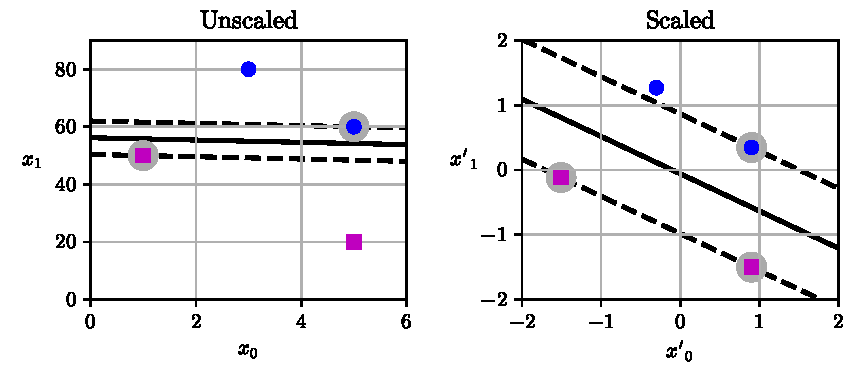
\includegraphics[width=\textwidth]{images/MachineLearning/LinearSVM.pdf}
    \caption{Linear SVM example \citepage{hands-on-geron2022}{176}}
    \label{fig:LinearSVM}
\end{figure}

Looking at \autoref{fig:LinearSVM}, it is possible to visualize what the algorithm does: it finds the plane that separates one class from the other, and vice-versa for the second class. In other words, it finds the most distant parallel hyperplanes that separate the two classes. As evident from the figure, the distance between the hyperplanes (called \emph{margin}) is sensitive to the features scaling. The term \quoted{support} derives from the fact that only the instances that are on the margin, define (support) the two planes. Those instances are called \emph{support vectors}, and in the figure are highlighted with a grey circle.

\subsubsection{Noninear \gls{svm}}
\label{subsubsec:NoninearSVM}
As said before, the \gls{svm} algorithm can be used also for nonlinearly separable data, using the \emph{kernel trick}. The idea is to project the data into a higher dimensional space, where they are linearly separable, and then use the linear \gls{svm} algorithm. The projection is done using a \emph{kernel mapping}. 

Let's have a look at what is the function for classifying an instance $\vect{x}^{(i)}$:
\begin{equation}
    t^{(i)} = \begin{cases}
        -1 & \text{if } \vect{w}^T\vect{x}^{(i)} + b < 0 \\
        1 & \text{if } \vect{w}^T\vect{x}^{(i)} + b \geq 0 
    \end{cases}
\end{equation}

The model is trainded to find the parameters $\vect{w}$ and $b$ that:
\begin{align}
    \label{eq:LinearSVM}
    \underset{\vect{w},b}{\text{minimize }} & \frac{1}{2}\vect{w}^T\vect{w} \\
    \text{subject to } & t^{(i)}(\vect{w}^T\vect{x}^{(i)} + b) \geq 1 \quad \forall i = 1, \dots, m
\end{align}

Since the objective function is convex, and the inequality constraints are differentiable and convex, the solution is the same as the solution of the dual problem \citepage{hands-on-geron2022}{188}:
\begin{align}
    \label{eq:LinearSVMdual}
    \underset{\vect{\alpha}}{\text{minimize }} & \frac{1}{2}\sum_{i=1}^{m}\sum_{j=1}^{m}\alpha^{(i)}\alpha^{(j)}t^{(i)}t^{(j)}\vect{x}^{(i)T}\vect{x}^{(j)} -\sum_{i=1}^{m}\alpha^{(i)}\\
    \text{subject to } & \alpha^{(i)} \geq 0 \quad \forall i = 1, \dots, m \quad \text{and} \quad \sum_{i=1}^{m}\alpha^{(i)}t^{(i)}=0
\end{align}

\paragraph{Kernel Trick}
Suppose wanting to use a second degree polynomial mapping, the mapping function is defined as:
\begin{equation}
    \phi(\vect{x}) = \phi(\begin{bmatrix}
        x_1 \\
        x_2 \\
    \end{bmatrix}) = \begin{bmatrix}
        x_1^2 \\
        \sqrt{2}x_1x_2 \\
        x_2^2 \\
    \end{bmatrix}
\end{equation}

Trasforming two vectors $\vect{a}$ and $\vect{b}$ with the mapping function, to be inserted in \autoref{eq:LinearSVMdual}:
\begin{equation}
    \phi(\vect{a})^T\phi(\vect{b}) = \begin{bmatrix}
        a_1^2 \\
        \sqrt{2}a_1a_2 \\
        a_2^2 \\
    \end{bmatrix}^T
    \begin{bmatrix}
        b_1^2 \\
        \sqrt{2}b_1b_2 \\
        b_2^2 \\
    \end{bmatrix} = a_1^2b_1^2 + 2a_1b_1a_2b_2 + a_2^2b_2^2 = (\vect{a}^T\vect{b})^2
\end{equation}

So, trasforming with a polynomial mapping of degree $d$, does not require to compute the mapping function, but just to compute the dot product of the two vectors and elevate it to the degree $d$, in the dual problem. There also are other kind of kernels, resumed in the following:
\begin{align*}
    \text{Linear: } & K(\vect{a}, \vect{b}) = \vect{a}^T\vect{b} \\
    \text{Polynomial: } & K(\vect{a}, \vect{b}) = (\gamma\vect{a}^T\vect{b} + r)^d \\
    \text{Gaussian RBF: } & K(\vect{a}, \vect{b}) = \exp(-\gamma\norm{\vect{a}-\vect{b}}^2) \\
    \text{Sigmoid: } & K(\vect{a}, \vect{b}) = \tanh(\gamma\vect{a}^T\vect{b} + r)
\end{align*}

\begin{figure}
    \centering
    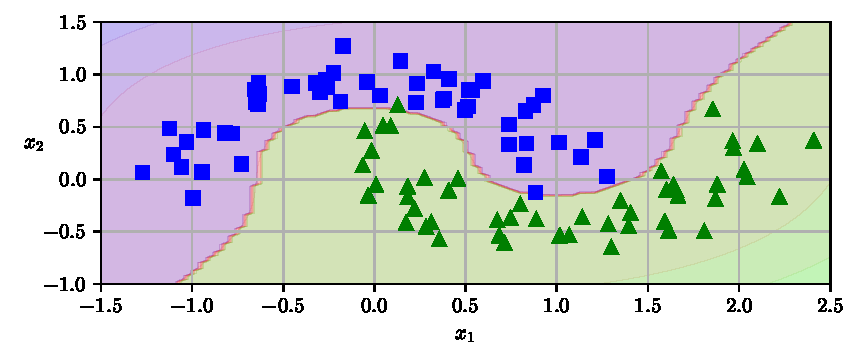
\includegraphics{images/MachineLearning/KernelTrick.pdf}
    \caption{Kernel Trick example \citepage{hands-on-geron2022}{180}}
    \label{fig:KernelTrick}
\end{figure}

The \autoref{fig:KernelTrick} shows an example of \gls{svm} classification of data that are not linearly separable.

This topic seems unrelated to the scope of this thesis, but in \autoref{sec:OneClassSupportVectorMachine} we will see how to use the \gls{svm} algorithm for novelty detection, as a one class classifier.


\subsection{Decision Trees \gls{dt}}
\label{subsec:dt}

\begin{figure}
    \centering
    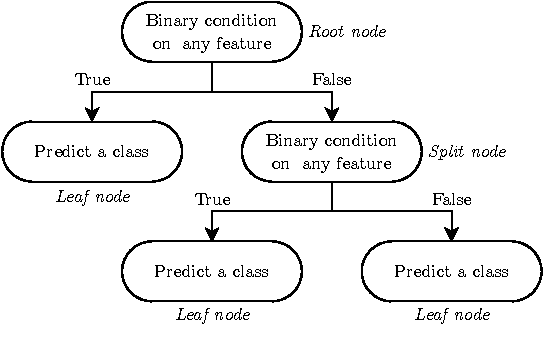
\includegraphics[scale = 1]{images/MachineLearning/DT_structure.pdf}
    \caption{Decision Tree structure}
    \label{fig:DecisionTree}
\end{figure}

Decision Trees are very powerful classification algorithms that can also be used for regression, thinking as a feature values as classes. The classification process is based on a tree structure, where each sample start from the root node, and is filtered thru a bunch of \emph{if - then} statement until it reaches a leaf node, that output the predicited class. In \autoref{fig:DecisionTree}, it is illustrated the structure of a very simple binary tree with only a split node and three leaf nodes.

\paragraph*{Gini impurity}
The classification algorithm is hence very simple, the \gls{ml} part of is the training process. Let's consider a leaf node, and imagine passing all the training samples thru the tree. Ideally, all the samples that reach the leaf node (and any other leaf node) should have the same class. This is possible, but a tree that does that is most likely very overfitted to the train dataset and will not perfom well on future data. Anyway, the aim of training is to obtain a tree close enough to the ideal one, without overfitting. To do that, it exist a metric called \emph{Gini impurity} that assume a value of zero if the leaf node is pure (all the samples that reach it have the same class), or a positive value $\in (0,0.5]$ that measure how different the classes in the node are, 0.5 being the maximum value that mean that all the classes are present in the node with equal frequency. The mathematical definition is the following:
\begin{equation}
    G_i = 1 - \sum_{k=1}^{n}p_{i,k}^2
\end{equation}
where $p_{i,k}$ is the ratio of class $k$ instances among the training instances in the $i^{th}$ node.

Then the training procedure tries to grow a tree defining the binary conditions that minimize the weighted average of the Gini impurity of the two child nodes, so the cost function is:
\begin{equation}
    J(k, t_k) = \frac{m_{\text{left}}}{m}G_{\text{left}} + \frac{m_{\text{right}}}{m}G_{\text{right}}
\end{equation}
where $k$ is the feature index, $t_k$ is the threshold value, $m_{\text{left}}$ and $m_{\text{right}}$ are the number of instances in the left and right child nodes, and $G_{\text{left}}$ and $G_{\text{right}}$ are the Gini impurity of the left and right child nodes.

A common way for minimization of the cost function is to use the \emph{Classification and Regression Tree} (\gls{cart}) algorithm, that is a greedy algorithm that search for the optimal split at each node, but not for the global optimal tree. The algorithm complexity is $\mathcal{O}(n \times m \log_2(m))$.

\paragraph{Entropy}
Another metric that can be used instead of Gini impurity inside the same cost function is the \emph{entropy} of the node, that is defined as:
\begin{equation}
    H_i = - \sum_{k=1}^{n}p_{i,k}\log_2(p_{i,k})
\end{equation}

This renders trees very similar to the ones obtained using Gini impurity, but the entropy is slightly slower to compute, due to the logarithm. however, it tends to produce slightly more balanced trees \cite{raschka2013decisiontrees}.

\paragraph{Avoid overfitting}
To avoid overfitting the data, the \gls{cart} algorithm implementation in \texttt{sklearn} has some \gls{glo:hyperparameter}s that can be tuned:
\begin{itemize}
    \item \texttt{max\_depth}: the maximum depth of the tree;
    \item \texttt{min\_samples\_split}: the minimum number of samples a node must have before it can be split;
    \item \texttt{min\_samples\_leaf}: the minimum number of samples a leaf node must have;
    \item \texttt{max\_leaf\_nodes}: the maximum number of leaf nodes;
    \item \texttt{max\_features}: the maximum number of features that are evaluated for splitting at each node.
\end{itemize}
Increasing the \texttt{min} bound, or decreasing the \texttt{max} bound, will regularize the model, and reduce the risk of overfitting.
In \autoref{fig:DecisionTreeOverfitting} it is shown an example of overfitting, where the left plot shows the decision boundaries of a tree with no regularization, and the right plot shows the decision boundaries of a tree with regularization.

\begin{figure}
    \centering
    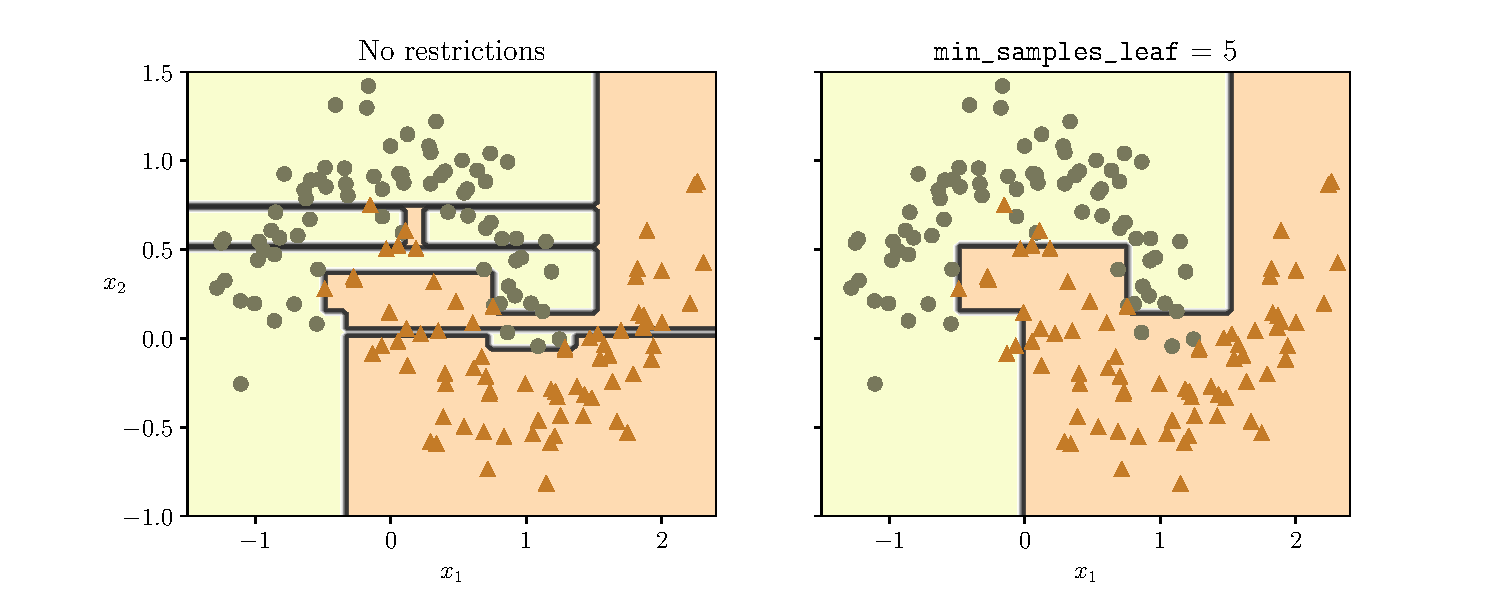
\includegraphics{images/MachineLearning/DecisionTreeOverfitting.pdf}
    \caption{Decision Tree overfitting example \citepage{hands-on-geron2022}{203}}
    \label{fig:DecisionTreeOverfitting}
\end{figure}

\paragraph{Regression}
As anticipated, the \gls{dt}s can also be used for regression, in this case, the cost function is the \gls{mse} of the predicted value in the leaf node:
\begin{equation}
    J(k, t_k) = \frac{m_{\text{left}}}{m}\text{MSE}_{\text{left}} + \frac{m_{\text{right}}}{m}\text{MSE}_{\text{right}}
\end{equation}

\paragraph{Advantages and limitations}
The main disadvantages of \gls{dt}s are that the classification proedure uses thresholds on the features value (cutting the hyperspace in orthogonal hyperplanes), so they are sensitive to axis orientation, and they are very sensitive to small variations in the training data. They are also very sensitive to the \gls{glo:hyperparameter}s, so a small caiations in constraints leads to very different trees. The main advantages are that they are very fast to train, and the resulting model is very fast to make predictions, they are very easy to understand and visualize and they do not require any feature scaling or centering.

\subsection{Random Forests \gls{rf}}
\label{subsec:rf}
The high sensituvity of the \gls{dt}s to small variations in the training data, can be reduced using the \emph{Random Forests} (\gls{rf}) algorithm. The idea is to train a bunch of \gls{dt}s on different random subsets of the training data, and then to average their predictions. The subsets of the training set are usually picked randomly with replacement, this technique is called \emph{bagging} (short for \emph{bootstrap aggregating}). 

The benefits of using more threes on subset of the training data are shown in the \autoref{fig:RandomForest}. The left plot shows the decision boundaries of a single \gls{dt}, the center plot shows the decision boundaries of a \gls{rf} with 500 trees.

\begin{figure}
    \centering
    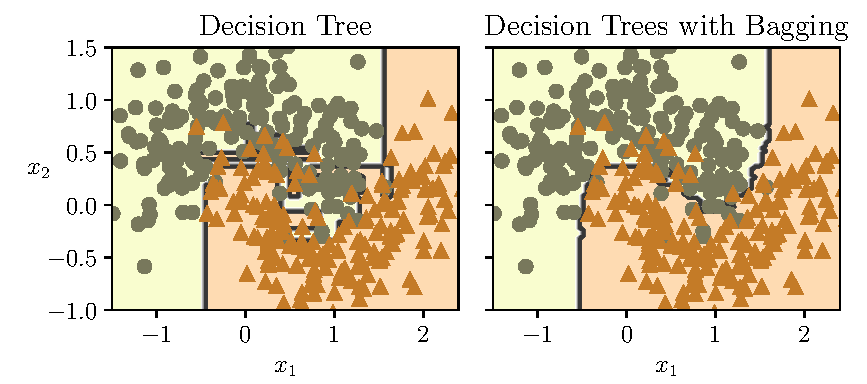
\includegraphics{images/MachineLearning/RandomForest.pdf}
    \caption{Random Forest example \citepage{hands-on-geron2022}{218}}
    \label{fig:RandomForest}
\end{figure}

Again, this topic seems unrelated to the scope of this thesis, but in \autoref{sec:IsolationForest} we will see how to use the \gls{rf} algorithm for novelty detection, exploiting the fact that outliers are usually more isolated (require more split nodes to be rached) than the normal instances.